%%%%%%%%%%%%%%%%%%%%%%%%%%%%%%%%%%%
% Results
%%%%%%%%%%%%%%%%%%%%%%%%%%%%%%%%%%%

\section{Results and Evaluation}


\subsection{Data set sizes}
Using a computer with only 8GB of memory a 16GB file with 2,621,440,000 records ran successfully, due to time constraints it's difficult to say with certainty that significantly larger files will work. When talking about hundreds of GBs or TBs of data then it is likely that a distributed system will be used, not a shared-memory system.

\subsection{Comparisons}

\subsubsection{Parallel vs Sequential}
As can be seen in Figure \ref{speedup}, there is a lack of speed up when running the same data set in parallel and sequential. We tested each problem in parallel on both CPU and GPU, and found that using the GPU was significantly faster, so our results are from the GPU. Parallel run time is consistently higher than sequential, with times converging with larger datasets. The main factor causing OpenCL to run slower was that the overhead of setting the device up and transferring the data far outweighs the benefit of running the calculations on a compute device. Running these computations with OpenMP would provide the needed speed up and due to the problem structure it would also suit OpenMP more than OpenCL. When operating on the same dataset, changing work group size had minimal effects. We believe this is again due to the overhead of transferring data. As the same amount of data will be needed to have been transferred no matter the work group size, it far outweighes the small benefit of changing the work group size \cite{Karimi2015}. 


\begin{figure}[H] \label{speedup}
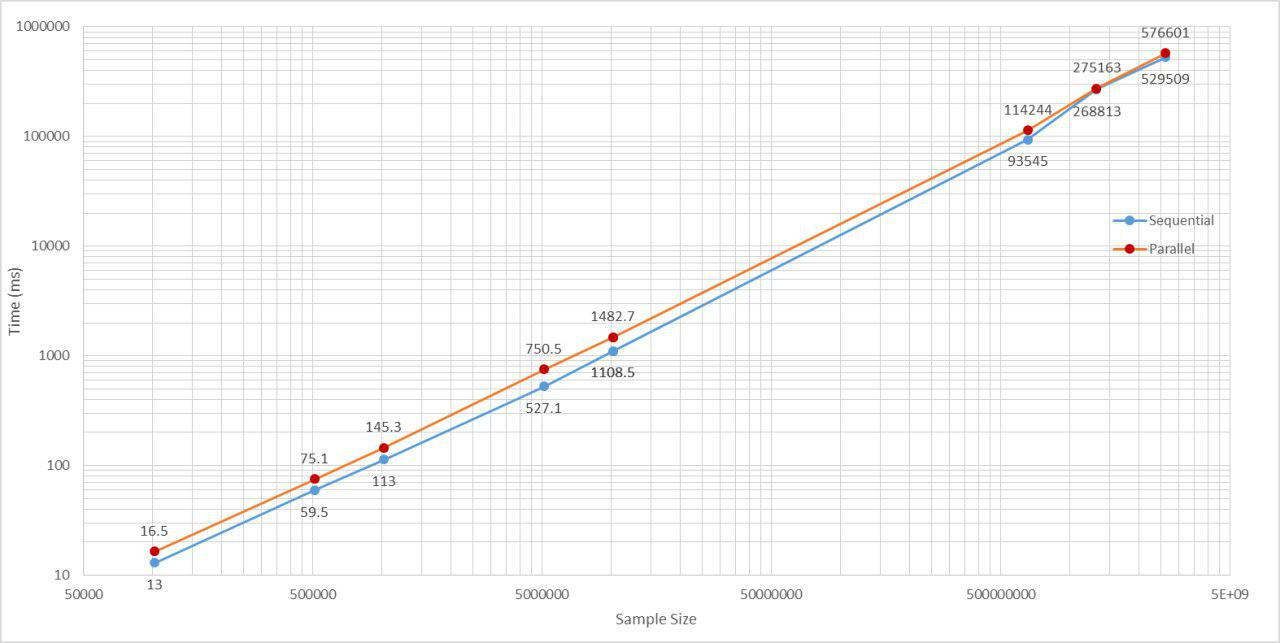
\includegraphics[width=\linewidth]{images/big-graph.jpg}
\caption{Sequential vs Parallel with different data set sizes}
\end{figure}

\subsubsection{MATLAB}
We had issues creating dataset files greater than 4GB because even 64-bit MATLAB wouldn't allocate that much memory on the heap. To generate larger files we had to concatenate the 4GB file with \texttt{cat}. MATLAB is also affected by \texttt{double} representation error in the same way and its complexity caused CSV reading to be longer.

\subsubsection{Other}
The most popular packages for analysis of large datasets are statistical programs such as Microsoft Excel, SAS or R. Excel is limited by spreadsheet size and thus is limited to approx 1million rows of data. SAS has limits on local-data imports of 4GB. The recommended approaches for using data sets larger than these on desktop programs is to split the input into multiple files. The 32-bit version of R has a limit of $2^{32} - 1$ vector length which is the same order of size as we tested with our program. R also supports using single-file large data sets; however, it employs big-data concepts that were beyond the scope of this project.
